\documentclass[11pt, english]{article}
\usepackage{graphicx}
\usepackage[colorlinks=true, linkcolor=blue]{hyperref}
\usepackage[russian,english]{babel}
\selectlanguage{russian}
\usepackage[utf8]{inputenc}
\usepackage[svgnames]{xcolor}
\usepackage{amsmath}

\usepackage{listings}
\usepackage{afterpage}
\pagestyle{plain}

\definecolor{dkgreen}{rgb}{0,0.6,0}
\definecolor{gray}{rgb}{0.5,0.5,0.5}
\definecolor{mauve}{rgb}{0.58,0,0.82}

% \lstset{language=R,
%     basicstyle=\small\ttfamily,
%   stringstyle=\color{DarkGreen},
%     otherkeywords={0,1,2,3,4,5,6,7,8,9},
%     morekeywords={TRUE,FALSE},
%     deletekeywords={data,frame,length,as,character},
%     keywordstyle=\color{blue},
%     commentstyle=\color{DarkGreen},
% }

\lstset{frame=tb,
language=java,
aboveskip=3mm,
belowskip=3mm,
showstringspaces=false,
columns=flexible,
numbers=none,
keywordstyle=\color{blue},
numberstyle=\tiny\color{gray},
commentstyle=\color{dkgreen},
stringstyle=\color{mauve},
breaklines=true,
breakatwhitespace=true,
tabsize=3
}

\usepackage{here}


\textheight=21cm
\textwidth=17cm
%\topmargin=-1cm
\oddsidemargin=0cm
\parindent=0mm
\pagestyle{plain}

%%%%%%%%%%%%%%%%%%%%%%%%%%
% La siguiente instrucción pone el curso automáticamente%
%%%%%%%%%%%%%%%%%%%%%%%%%%

\usepackage{color}
\usepackage{ragged2e}

\global\let\date\relax
\newcounter{unomenos}
\setcounter{unomenos}{\number\year}
\addtocounter{unomenos}{-1}
\stepcounter{unomenos}
\gdef\@date{\arabic{unomenos}}

\begin{document}

\begin{titlepage}

\begin{center}
\vspace*{-1in}
\begin{figure}[htb]
\begin{center}

\includegraphics[width=8cm]{bw_w_rus.png}
\end{center}
\end{figure}

Факультет Программной Инженерии и Компьютерных Технологий - \@date\\
\vspace*{0.15in}
Вычислительная математика \\
\vspace*{0.4in}
\begin{large}
ЛАБОРАТОРНАЯ РАБОТА №2:\\
\end{large}
\vspace*{0.2in}
\begin{Large}
\textbf{Интегрирование} \\
\end{Large}
\vspace*{0.3in}
\begin{large}
Метод симпсона \\
\end{large}
\vspace*{0.3in}
\rule{80mm}{0.1mm}\\
\vspace*{0.1in}
\begin{large}
Преподаватель: Перл О.В. \\
Выполнил: Куприянов А.А, P3212 \\
\end{large}
\vspace*{1.5in}
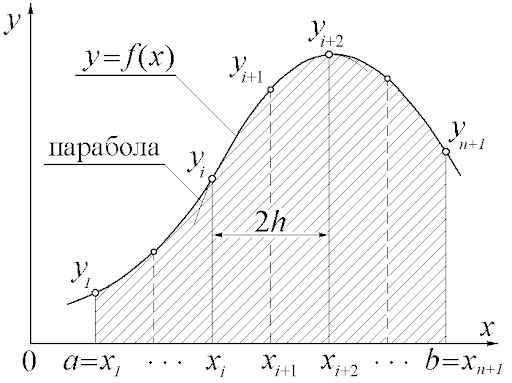
\includegraphics[width=7cm]{unnamed.png}
\end{center}
\end{titlepage}

\newcommand{\CC}{C\nolinebreak\hspace{-.05em}\raisebox{.4ex}{\tiny\bf +}\nolinebreak\hspace{-.10em}\raisebox{.4ex}{\tiny\bf +}}
\def\CC{{C\nolinebreak[4]\hspace{-.05em}\raisebox{.4ex}{\tiny\bf ++}}}


\section{Теория}

Метод симпсона - численный метод интегрирования, суть которого заключается в приближении графика функции на определенном отрезке параболой.\\

Основой метода симпсона является разбиение подынтегральной функции на несколько частей, а затем вычисление площади каждой из частей как криволинейной трапеции, ограниченной сверху параболой

\begin{center}
\begin{figure}[h!]
    \centering
    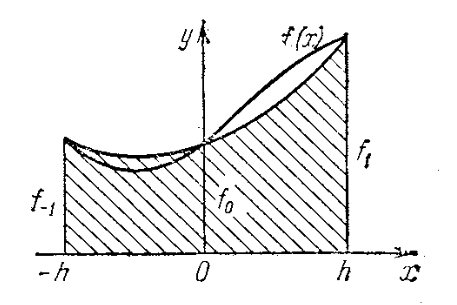
\includegraphics[width=7cm]{FS4iqxg.png}
    \caption{Криволинейная трапеция}
    \label{fig:my_label}
\end{figure}
    
\end{center}

Очевидно, что чем больше количество частей на которые разбивается подынтегральная функция, тем больше точность, так как не смотря на то, что используется парабола - это все равно интерполяционный многочлен.\\

Таким образом, можно получить необходимую точность путем задания количества разбиений.

\section{Формула Симпсона}
Рассмотрим рисунок 1. В ней трапеция ограничена параболой проходящей через точки ($-h, f_{-1}$), ($0, f_0$), ($h, f_1$), где $f_i = f(ih)$

Уравнение указанной параболы:
$$y = f_0 + \frac{f_1 - f_{-1}}{2h} x + \frac{f_{-1} - 2f_0 + f_1}{2h^2} x^2$$

Отсюда находим:
$$\int_{-h}^h y dx = \frac{h}{3}(f_{-1} + 4f_0 + f_1)$$

Из интересного можно заметить, что точка ($0, f_0$) в 4 раза весомее каждой из двух своих соседей\\

Таким образом, формула Симпсона имеет вид:
$$\int_{-h}^h f(x) dx \approx \frac{h}{3}(f_{-1} + 4f_0 + f_1)$$


\subsection{Приближенное вычисление интеграла}

Для использования этой формулы для численного метода нам необходимо знать отрезок интегрирования и количество частей, на которые будет делиться подынтегральная функция.\\

С другой стороны, пользователь не заинтересован в количестве разбиений - его интересует точность вычислений. Поэтому разумно будет дать пользовтелю ввод точности и в зависимости от этих данных вычислить количество разбиений. \\

Для этого в лабораторной работе было предложено использование оценки погрешности с помощью правила Рунге.\\

Суть его заключается в том, чтобы сравнить найденное значение с разбиением в два раза меньшим, чем с текущим.
$$I - I_{h/2} \approx \frac{I_{h/2} - I_h}{2^k - 1}$$

Так как значение точности вычисляется в ходе выполнения программы, то мы можем сами задать начальное рабиение, и дальше увеличивать его в двое.

\section{Функции для вычисления}
Для этой лабораторной работы было выбрано 5 функций. Одно уравнение второго порядка и остальные 4 имеющие разрыв функции.

\subsection{Уравнение второго порядка}
$$f(x) = x^2 - 1$$
\begin{center}
    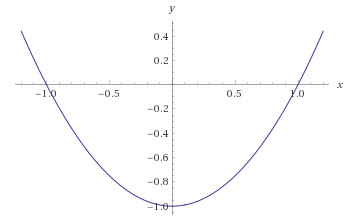
\includegraphics[width=7cm]{2-func.png}
\end{center}

Неразрывная функция

\subsection{Уравнения с разрывами}
\begin{center}
    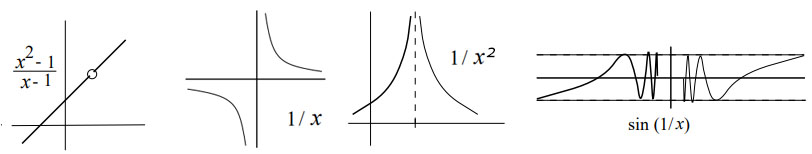
\includegraphics[width=15cm]{functions.jpg}
\end{center}

\subsubsection{$$\frac{x^2 - 1}{x - 1}$$}

В первом уравнении, при $x = 1$ мы получаем деление на $0$. Тем не менее, мы можем написать так:
$$\frac{x^2 - 1}{x - 1} = \frac{(x+1)(x-1)}{x-1} = x + 1$$

Так, мы получаем кусочно-заданную функцию (Piecewise)

\[ \begin{cases} 
      2 & x = 1 \\
      \frac{x^2 - 1}{x - 1} & x \neq 1 \\
   \end{cases}
\]

\subsubsection{$$1/x$$}
Эта функция имеет точку разрыва при $x = 0$. Функция непрерывна на $(-\infty, 0)$ и на $(0, \infty)$, для $x < 0$ и $x > 0$

Но это четная функция и симметричная относительно оси ординат. 
$$\lim_{x \rightarrow 0^+} \frac{1}{x} = + \infty$$
$$\lim_{x \rightarrow 0^-} \frac{1}{x} = - \infty$$

Следовательно, мы можем доопределить промежуток интегрирования, в том случае, если ни один из пределов интегрирования не равен $0$.

Аналогично решаем функцию $$sin(1/x)$$

\subsubsection{$$1/x^2$$}

Такую нечетную функцию уже нельзя доопределить и мы можем утверждать, что если в область интегрирования входит точка $x \rightarrow 0$, то получим бесконечность. 


\section{Программа}

Технические данные: Java 11, OpenJDK 11, OS: Windows Linux Subsystem \\

Пусть, $n$ - количество разбиений функции на части, при том, $n$ - четное, такое что каждое разбиение - имеет длину на оси $x$: $h/2$\\

При каждой итерации (кроме первой) мы будет сравнивать предыдущее найденное значение с $n/2$, таким образом вычисляя текущую точность.\\

Как ранее уже говорилось, средняя часть имеет вес в 4 раза больший, чем соседние. Тем не менее, соседние учитываются дважды (при вычислении соседнего разбиения).\\

Таким образом, в зависимости от четности порядкового номера мы можем раздельно их суммировать, а затем в результате умножить эту сумму на соответствущий коэффициент
\newpage
\begin{center}
\begin{figure}[h!]
    \centering
    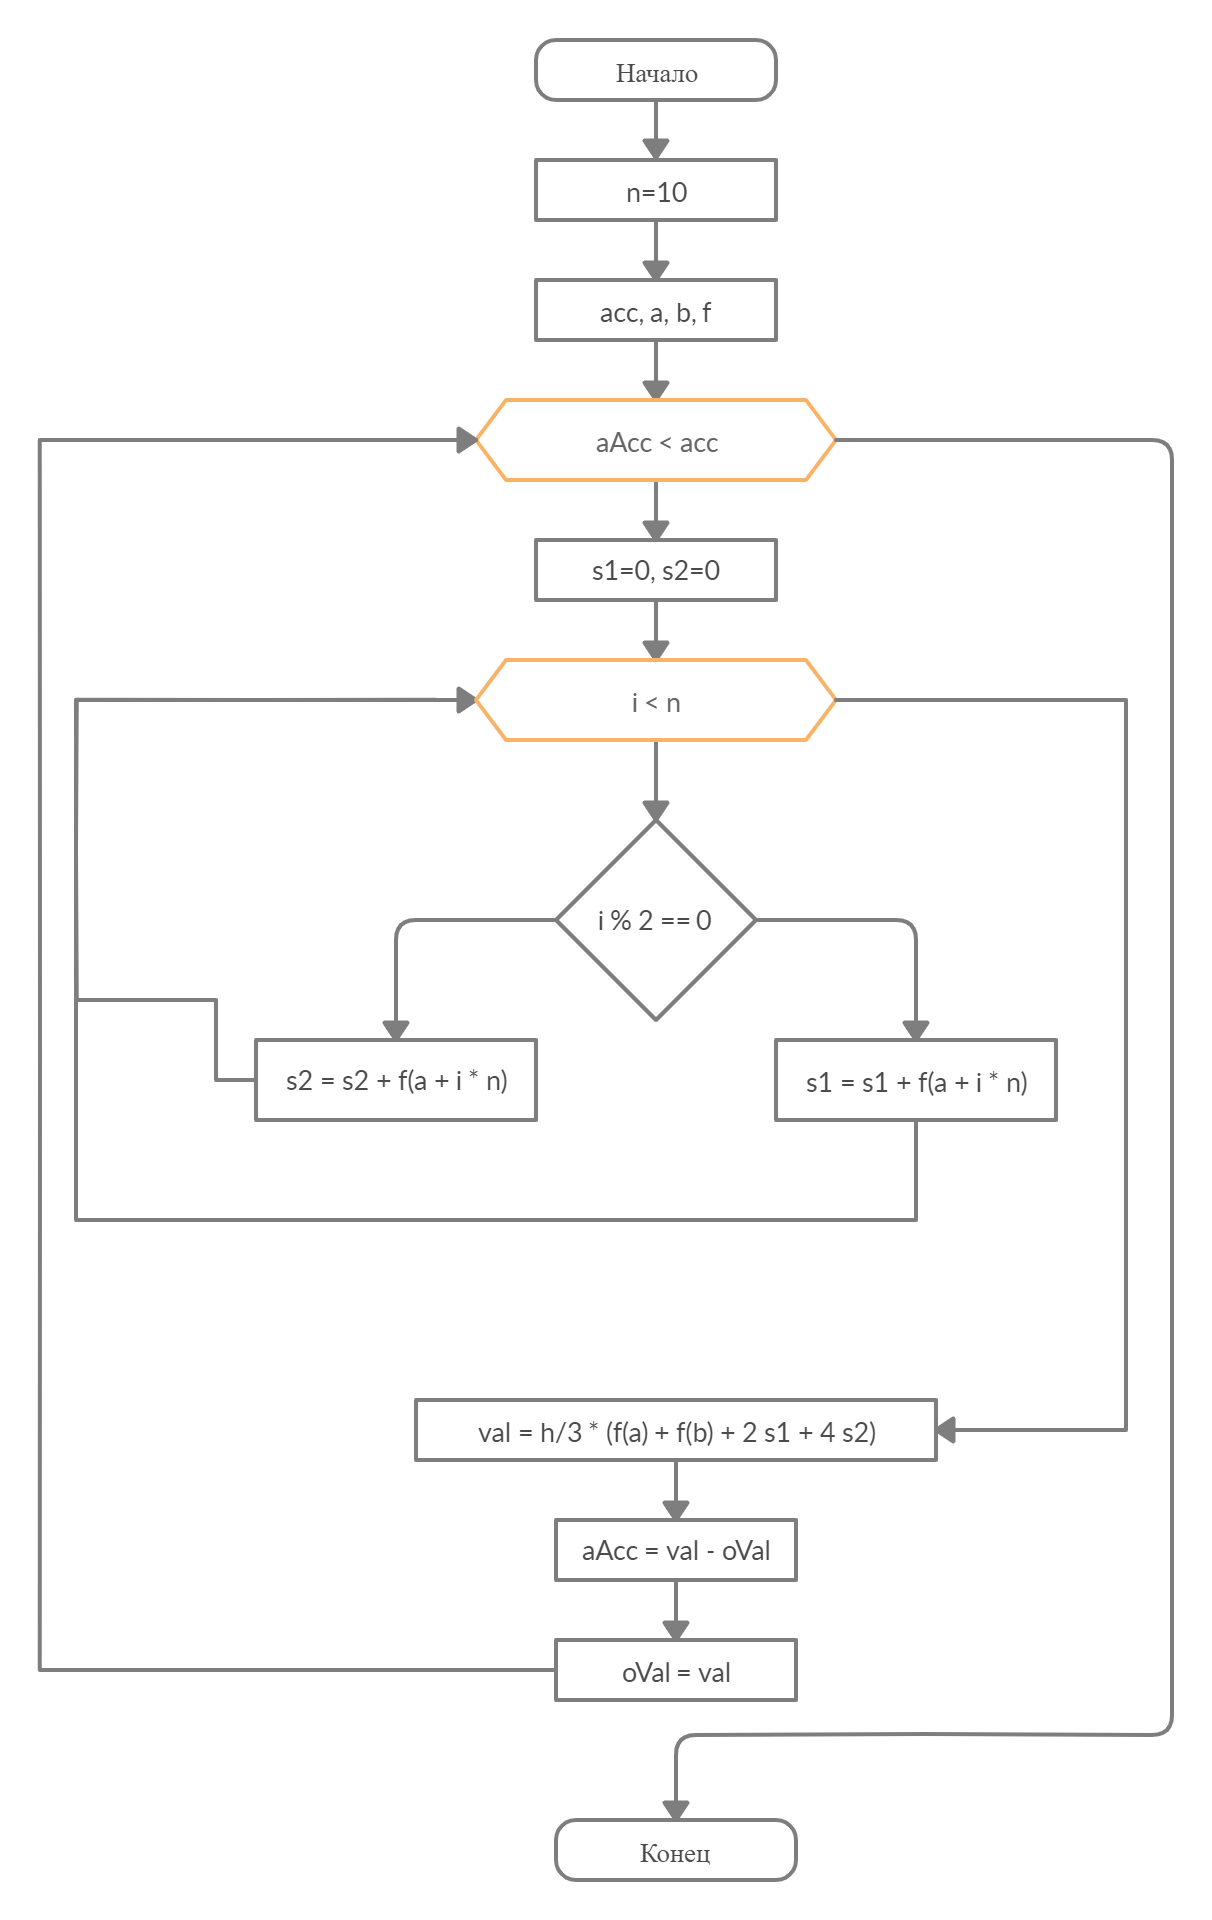
\includegraphics[width=12cm]{diagram.jpg}
    \caption{Диаграмма}
    \label{fig:my_label}
\end{figure}
\end{center}






\subsection{Реализация}


\begin{lstlisting}
public double solve(Function<Double, Double> function, int top, int bottom, int partition) {
    int[] boundaries = new int[2];
    addBoundariesTo(boundaries, top, bottom);

    double step = (boundaries[1] - boundaries[0] * 1d) / partition;

    double sum1 = 0;
    double sum2 = 0;

    for (int i = 0; i < partition; i++) {
        double functionValue = function.apply(boundaries[0] + i * step);
        if (i % 2 == 0) {
            sum1 = sum1 + functionValue;
        } else {
            sum2 = sum2 + functionValue;
        }
    }
    byte sign = (byte) (top > bottom ? 1 : -1);
    return sign * step / 3 * (function.apply((double) boundaries[0]) + function.apply((double) boundaries[1]) + 2 * sum1 + 4 * sum2);
}
\end{lstlisting}
\begin{lstlisting}
public double solveWithAccuracy
(Function<Double, Double> function, int top, int bottom, double expectedAccuracy){
    int partition = 10;
    double actualAccuracy = Double.MAX_VALUE;
    double oldValue = solve(function, top, bottom, partition);
    while (actualAccuracy > expectedAccuracy) {

        partition = partition * 2;
        double actualValue = solve(function, top, bottom, partition);
        actualAccuracy = Math.abs(actualValue - oldValue) / 15;
        oldValue = actualValue;

    }
    lastAccuracy = actualAccuracy;
    lastPartition = partition;
    return oldValue;
}
\end{lstlisting}

\newpage

\section{Заключение}

Зачастую метод Симпсона точнее остальных методов через квадратурные формулы прямоугольников или трацеций. Это вызвано тем, что для интерполяции используется многочлен второго порядка, который дает более точное приближение, чем остальные (в зависимости от подынтегральной функции). Но также основным плюсом данного метода является безусловно формула Симсона, которая упрощает вычисление интерполированного интеграла путем сведения его к одной формуле. \\

Из плюсов также можно отметить, то что мы имеем контроль точности, а следовательно можем экономить вычислительные мощности по мере возможности. \\

Хоть и формулы прямоугольников и трапеций по отдельности уступают формуле Симпсона при интегрировании "гладких" функций, но в паре они могут дать двустороннее приближение интеграла. Но эта тема уже касается усложненных квадратурных формул. \\

А одним из минусов самого метода Симпсона является излишняя нагрузка ресурсов для вычисления, допустим, линейных функций, так как она в методе также будет интерполироваться в многочлен второй степени.

\end{document}